\documentclass{article}%
\usepackage[T1]{fontenc}%
\usepackage[utf8]{inputenc}%
\usepackage{lmodern}%
\usepackage{textcomp}%
\usepackage{lastpage}%
\usepackage[head=40pt,margin=0.5in,bottom=0.6in]{geometry}%
\usepackage{graphicx}%
%
\title{\textbf{Trabajadores de Ferrominera de Guayana exigen aumento de sueldo}}%
\author{El Nacional Web}%
\date{22/11/2018}%
%
\begin{document}%
\normalsize%
\maketitle%
\textbf{URL: }%
http://www.el{-}nacional.com/noticias/protestas/trabajadores{-}ferrominera{-}guayana{-}exigen{-}aumento{-}sueldo\_260707\newline%
%
\textbf{Periodico: }%
EN, %
ID: %
260707, %
Seccion: %
Protestas\newline%
%
\textbf{Palabras Claves: }%
Nicolás Maduro, Economía, Protestas, Sociedad, Inflación\newline%
%
\textbf{Derecho: }%
2.3%
, Otros Derechos: %
NO\_TIENE%
, Sub Derechos: %
2.3.4%
\newline%
%
\textbf{EP: }%
NO\newline%
\newline%
%
\textbf{\textit{Aseguran que el único regalo que los venezolanos quieren es la salida del poder del presidente Nicolás Maduro}}%
\newline%
\newline%
%
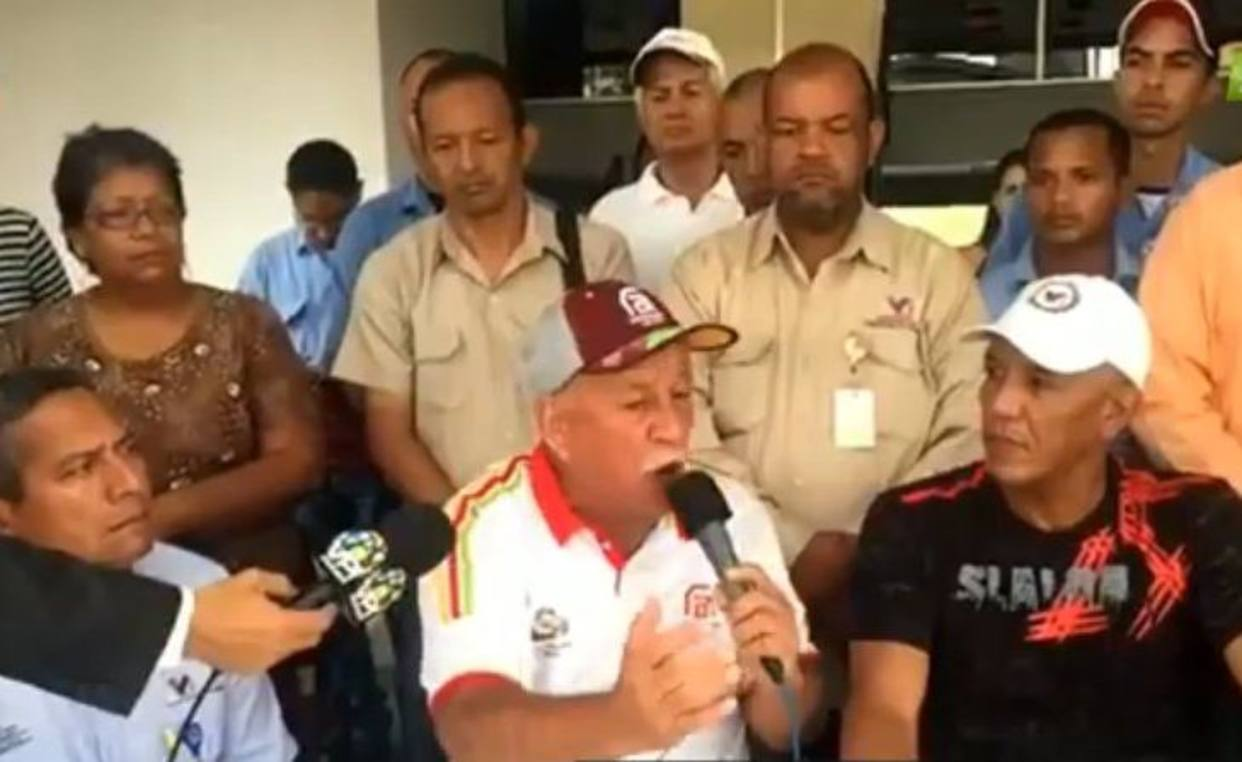
\includegraphics[width=300px]{108.jpg}%
\newline%
%
Un grupo de trabajadores de la Ferrominera, en Guayana, realizaron una rueda de prensa para exigir respeto a los salarios y a los contratos de la empresa.%
\newline%
%
Entre las exigencias~también está~una bonificación para poder comprar juguetes para sus hijos en la época decembrina.%
\newline%
%
Además, los empleados pidieron la salida del presidente Nicolás Maduro del poder.%
\newline%
%
“El único regalo que los trabajadores y todo el pueblo venezolano le pide a Maduro es que se vaya, que abandone el poder porque le quedo grande”, dijo Rubén González, presidente del sindicato de la empresa.%
\newline%
%
Por otro lado, los trabajadores rechazaron las acciones cometidas por funcionarios de la Policía Nacional Bolivariana (PNB)~y de la Guardia Nacional Bolivariana (GNB) durante las protestas que han realizado.%
\newline%
%
\end{document}